\documentclass[10pt,conference ]{IEEEtran}

\input{input.tex}

\title{FederationS: Federated Learning for Spatial Reuse in a multi-BSS scenario}

\author{
    Jernej Hribar and Andrea Bonfante\\ 
    \\ The authors are with CONNECT Centre, Trinity College Dublin, Ireland
    \\ email: \{jhribar,bonfanta\}@tcd.ie
    %\thanks{Author~1, Author~2 are with CONNECT Centre, Trinity College Dublin, Ireland (e-mail: ).}
    }%

\begin{acronym}[mmWave-BSs] % Give the longest label here so that the list is nicely aligned
\acro{10GE}{10 Gigabit Ethernet}
\acro{3D}{Three-dimensional}
\acro{3GPP}{Third Generation Partnership Project}
\acro{5G}{5-th Generation}
\acro{AC}{Access}
\acro{ACK}{Acknowledgment }
\acro{Adam}{ADAptive Moment estimation}
\acro{AGV}{Automatic Guided Vehicle}
\acro{AoA}{Angle of Arrival}
\acro{AP}{Access Point}
\acro{AoD}{Angle of Departure}
\acro{AR}{Augmented Reality}
\acro{BER}{Bit Error Rate}
\acro{BF}{Beamforming}
\acro{BH}{Backhaul}
\acro{BLAS}{Basic Linear Algebra Subprograms}
\acro{BS}{Base Station}
\acro{BSS}{Basic Service Set}
\acro{CDF}{cumulative distribution function}
\acro{CP}{Cyclic Prefix}
\acro{CPU}{Central Processing Unit }
\acro{CSI}{Channel State Information}
\acro{DL}{Downlink}
\acro{DNN}{Deep Neural Network}
\acro{DoA}{Direction of Arrival}
\acro{DoD}{Direction of Departure}
\acro{DSP}{Digital Signal Processor}
\acro{DAPS}{Dual Active Protocol Stack}
\acro{E2E}{End-to-end}
\acro{eMBB}{Enhanced Mobile BroadBand}
\acro{FFT}{Fast Fourier Transform}
\acro{FN}{False Negative}
\acro{FP}{False Positive}
\acro{FPGA}{Field-Programmable Gate Array}
\acro{GT}{Ground Truth}
\acro{HD}{Half-Duplex}
\acro{HetNet}{Heterogeneos Network}
\acro{HO}{handover}
\acro{HW}{Hardware}
\acro{IA}{Initial Access}
\acro{IID}{Independent and Identically Distributed}
\acro{ISD}{Inter Site Distance}
\acro{L3}{Layer 3}
\acro{LoS}{Line-of-Sight}
\acro{LP}{Linear Program}
\acro{LSAS}{Large Scale Antenna System}
\acro{LTE}{Long Term Evolution}
\acro{MAC}{Medium Access Control}
\acro{MBB}{make-before-break}
\acro{MCS}{Modulation and Coding Scheme}
\acro{MILP}{Mixed Integer Linear Program}
\acro{MIMO}{Multiple-Input-Multiple-Output}
\acro{MKL}{Math Kernel Library}
\acro{ML}{Machine Learning}
\acro{MLP}{Multilayer Perceptron}
\acro{mmWave}{millimeter Wave}
\acro{mmWave-BS}{mmWave Base Station}
\acro{mmWave-BSs}{mmWave Base Stations}
\acro{MNO}{Mobile Network Operator}
\acro{MPC}{Multipath Components}
\acro{MWC}{Mobile World Congress}
\acro{NLoS}{Non Line-of-Sight}
\acro{NR}{New Radio}
\acro{OFDM}{Orthogonal Frequency Division Multiplexing}
\acro{OBSS}{Overlapping Basic Service Set}
\acro{PD}{Preamble Detection}
\acro{PHY}{Physical layer}
\acro{RAN}{Radio Access Network}
\acro{RACH}{Random-Access Channel}
\acro{RB}{Resource Block}
\acro{ReLu}{Rectified Linear unit}
\acro{RF}{Radio Frequency}
\acro{RLF}{Radio Link Failure}
\acro{RMSE}{Root Mean Square Error}
\acro{RSRP}{Reference Signal Received Power}
\acro{RSRP}{Reference Signal Received Power}
\acro{RSSI}{Received Signal Strength Indicator}
\acro{Rx}{Receiver}
\acro{SA}{standalone}
\acro{s-BH}{self-Backahuling}
\acro{SC}{small-cell}
\acro{SCM}{Spatial Channel Model}
\acro{SGD}{Stochastic Gradient Descent}
\acro{SINR}{signal to interference noise ratio}
\acro{SNR}{signal-to-noise ratio}
\acro{SSB}{synchronisation signal block}
\acro{STA}{station}
\acro{SVN}{Subversion}
\acro{SW}{Software}
\acro{TDD}{Time Division Duplex}
\acro{TI}{Texas Instruments}
\acro{TN}{True Negative}
\acro{TP}{True Positive}
\acro{TTI}{Transmission Time Interval}
\acro{Tx}{Transmitter}
\acro{UDP}{User Datagram Protocol}
\acro{UE}{User Equipment}
\acro{UL}{Uplink}
\acro{UPA}{Uniform Planar Array}
\acro{URLLC}{Ultra-Reliable Low-Latency Communication}
\acro{QoS}{Quality of Service}
\acro{RLC}{Radio Link Control}
\acro{RRC}{Radio Resource Control}
\acro{VR}{Virtual Reality}
\acro{WLAN}{Wireless Local Area Network}
\acro{FL}{Federated Learning}
\acro{GDPR}{General Data Protection Regulation}
\acro{MAE}{Mean Average Error}
\end{acronym}

\begin{document}
\maketitle

\begin{abstract}

\end{abstract}

\acresetall

\section{Data Analysis}\label{Sec: Data Analysis}


\begin{figure*}[t]
	\centering
	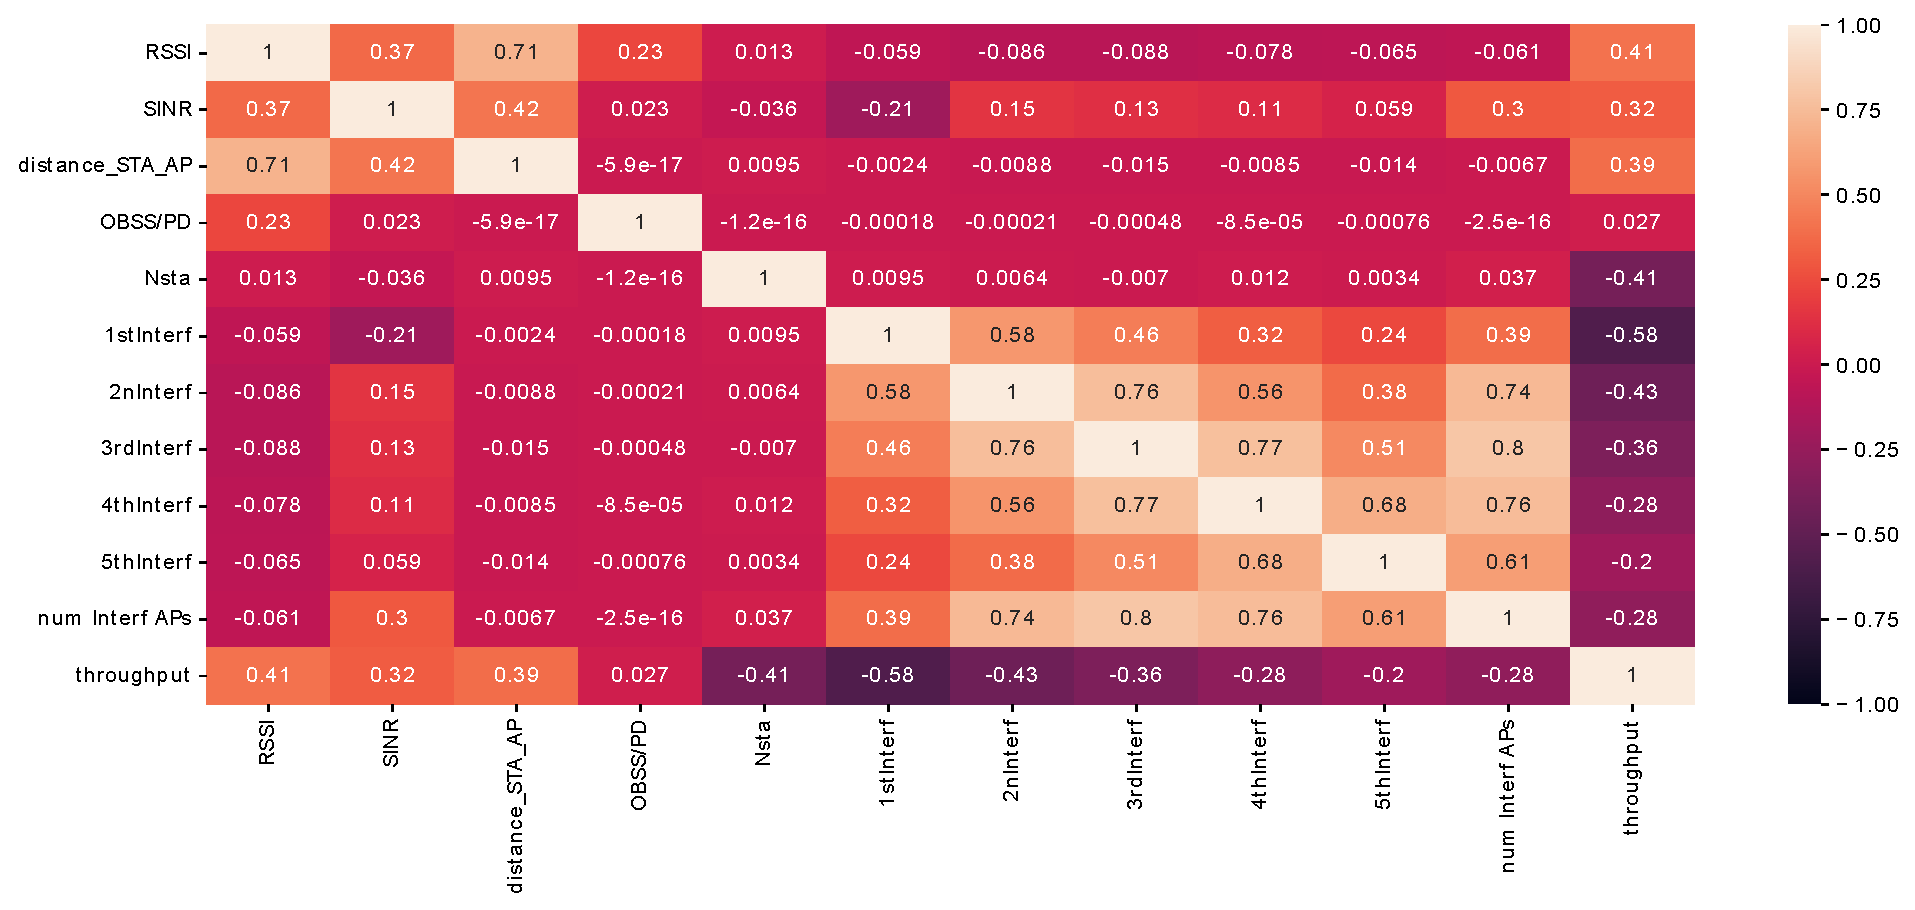
\includegraphics[width=\textwidth]{figures/Correlation_heatmap_r.eps}
	\caption{Representation of correlation matrix showing the correlation between different input and output variables of the dataset.}
	\label{fig:Correlation heatmap}
\end{figure*}

First, we discuss how features are selected for the training process. 
We use Version 1.3 of the dataset \cite{francesc_wilhelmi_2021_5506248} created for the problem statement ITU-ML5G-PS-004 of the ITU AI/ML Challenge (2021 edition). 
More specifically, we consider Scenarios 2 and 3, containing $2000$ different IEEE 802.11ax deployments with 2-6 \acp{AP} and 1-4 \acp{STA} per \ac{AP}. 
We start extracting the set of features available in the simulator's output file of each context, namely the \ac{OBSS}-\ac{PD} configuration, the \ac{RSSI}, the set of interference powers from other \acp{AP} sensed by the \ac{AP} in the reference \ac{BSS}, the \ac{SINR} and the throughput for each \ac{STA} served by the \ac{AP}.  
Then, we consider the additional information available in the simulator's input file of each context.
Here, we extract the coordinates of the \ac{AP} and the ones of the \ac{STA}. 
Then, we compute the Euclidean distances from each \ac{STA} to the serving \ac{AP}.
Moreover, we compute the number of \ac{STA} served by the \ac{AP} and the number of \acp{AP} interfering with the server \ac{AP} in the \ac{BSS} under analysis. 
It is worth noting that these information can also be obtained  online in a real system. Indeed, the \ac{RSSI}, \ac{SINR} and throughput measurements can be reported periodically by each \acp{STA}. 
Interference powers can be measured during the listen-before-transmit (LBT) phase at the \ac{AP}, employing multi-antenna processing techniques to separate the different interfering sources. 
In addition, Time-of-Arrival (TOA) ranging techniques can determine the distance between \ac{STA} and \ac{AP} . 

Before obtaining the final dataset, we preprocess the data through different steps. 
First, we clean the input and output data parsed from the simulator files removing all non-numerical values from the dataset.
Then, we arrange the data of each \ac{STA} to form 1-D vectors with $11$ numerical entries used as the input of the model and containing all measurements and system parameters. 
Conversely, we define the \ac{STA} throughput as the target variable and output of the model. 
To note that the features present entirely different ranges between maximum and minimum values and are expressed with different units of measurements, e.g. dBm for \ac{RSSI} and interference power, dB for \ac{SINR} and meters for distances. 
To balance each feature's contribution to the overall model predictions, we re-scale the features with the Min-Max normalisation method that transforms all features' in the range $[0,1]$. 
Finally, when input data are missing, like when the number of interfering \acp{AP} reported is less than the minimum recorded according to our system settings, we assign those values with $0$s. 
The activation function that we will explain later is chosen to keep neurons inactive when $0$s are present at the input. 

\begin{figure}[t]
	\centering
	\includestandalone[width=3.7in]{tikz_figures/ann_small}
	\caption{Visualisation of the DNN structure used.}
	\label{fig:DNN model}
	%\vspace{-10pt}
\end{figure}



The results of data preprocessing are shown in Fig. \ref{fig:Correlation heatmap}, where we represent the correlation matrix between input and output variables. 
Correlation values close to $0$ indicate a lack of relations and structure between the data corresponding to these variables, while correlation values close to $-1$ and $+1$ indicate a perfect negative and positive correlation between variables, respectively. 
Looking to Fig. \ref{fig:Correlation heatmap} two main observations can be made: 
\begin{enumerate}
\item Most features show a strong positive or negative correlation with the output variable (throughput). 
As expected, only the \ac{OBSS}-\ac{PD} feature does not directly affect the throughput. 
Otherwise, the problem would be trivial to model. 
Indeed, the \ac{OBSS}-\ac{PD} value is correlated to the \ac{RSSI} as discussed before, which affects \ac{SINR} and throughput variables, showing that relationships between input and output values of the system are not straightforward to characterise with domain-based models. 
This justifies the adoption of \ac{DNN}, which are extensively used for their capabilities to model nonlinear relationships. 
\item Two regions depicted with lighter colours  at the top left and at the bottom right of the correlation matrix identify two groups of features that show a strong positive correlation between input variables. 
Thus, in the \ac{DNN} architecture design, these inputs of the model need to be fully connected. 
In contrast, the two regions at the top right and bottom left are characterised by elements with close to zero correlation values, meaning that the relationship between features is not strong. 
Therefore, these connections are expected to bring a low contribution to the predictions and can be dropped in the \ac{DNN} architecture design. 
\end{enumerate}

\section{DNN Model Design}\label{Sec:Centralised Solution}
Based on the observations highlighted in Sec. \ref{Sec: Data Analysis}, we design the model architecture represented in Fig. \ref{fig:DNN model}.  
First, we split the \ac{DNN} model into two parallel branches. 
The inputs of the first branch are the features constituting the first block, i.e. \ac{RSSI}, \ac{SINR}, distance \ac{STA}-\ac{AP} and \ac{OBSS}-\ac{PD} threshold.
At the same time, features like the number of \ac{STA}, the power received from interfering \acp{AP} and the number of interfering \acp{AP} form the second block of features and are used as input of the second branch. 
The input layers are followed by two hidden layers defined for each branch separately. 
We use a concatenation layer to merge the output of these two branches. 

The result of the concatenation is then used as input of two additional hidden layers, which are connected to the output layer of the model. 
We adopt the hyperbolic tangent (\emph{tanh}) activation function to provide positive and negative outputs and keep neurons inactive when the inputs are $0$s. Finally, we add dropout layers after each layer before the output layer to reduce overfitting. 


\section{Federated Solution}\label{Sec: Federated Solution}
Our \ac{FL} solution is based on the implementation outlined in \cite{federated_repo}. 
In addition, our approach combines the trained weights in a novel way, which is designed specifically for this challenge and is based on the data acquired in each context. 

\subsection{The Proposed Solution}

Our proposed \ac{FL} solution follows the steps described in Algorithm \ref{alg:fed}. 
In steps 1-5, we initialize the contexts and split them into train and validation sets. 
After the initialization stage, the training takes place locally in a subset of $N_{tr}$ contexts, which are selected randomly at every communication epoch. 
The training results, i.e., the trained neural network $\theta_i$ and its weights $w_i$ along with the number of data sample $n_i$, are then transmitted from the $N_{tr}$ contexts to the central server for aggregation. 
After the aggregation, the central server sends back the global trained model to every context, which updates their local \ac{DNN} models. 
The training cycle repeats for $T$ communication epochs. 

One of the most important aspects of the \ac{FL} training consists of aggregating the weights at the central server. 
Initially, we weighted the updates from each context equally, but such an approach resulted in a skewed performance toward contexts with more \ac{STA}. Such behaviour can be attributed to the fact that contexts with four \ac{STA} have twice as many samples as contexts with only two \ac{STA}. 
Instead, our solution proposed to weight each context update based on the number of data samples used for the training in each context normalised by the number of \ac{STA} in the contexts. We denote this normalisation weights with $\alpha$. This approach improves the accuracy of the predictions of the throughput. 

\begin{algorithm}[]
 \caption{Proposed Federated Learning Solution.}
 \begin{algorithmic}[1]
    \State Initialise set $\mathbb{K}$,, i.e., init $K$ contexts with data samples
    \State From $\mathbb{K}$, select $N_{eval}$ to create $\mathbb{K}_{val}$
    \State Create a new set of contexts $\mathbb{K}_{tr} =  \mathbb{K} \cap \mathbb{K}_{val}$
    \State Server initialises model parameters $\theta^0$ and $W^0$
    \State The server transmits $\theta_k^0, w_k^0$ to $k$-th contexts
    \For{communication epoch $t=1,T$}
        \State Randomly select $N_{tr}$ contexts from $\mathbb{K}_{tr}$ to get $\mathbb{K}_{ep}$
        \For{$i$-th context in $\mathbb{K}_{ep}$}
        %\State The $i$-th context updates the model using %Adam Optimiser and MSE loss
        \State Split context's samples in $\beta$ ($\frac{n_i}{B}$ batches of size $B$)
        \State Where $n_i$ represents the number of data samples 
        \For{batch $b$ in $\beta$}
        \State  $\theta_i^t, w_i^t \leftarrow \theta_i^{t-1}, w_i^{t-1} - \eta \nabla l(\theta_i^{t-1}, w_i^{t-1};b)$
        \EndFor
        \State Determine weight $\alpha_i = n_i/N_{STA}$
        \State Transmit $\theta_i^t$, $w_i^t$, and $\alpha_i$ to central server
        \EndFor
        \State Calculate data samples weight $\alpha_{t} = \sum^{N_{tr}}_{i=1} \alpha_i$
        \State Update model: $\theta_k^t = \sum^{N_{tr}}_{i=1}  \frac{\alpha_i *\theta_i^t }{\alpha_t}$, $w_k^t = \sum^{N_{tr}}_{i=1}  \frac{\alpha_i w_i^t }{\alpha_t}$
        \State The server transmits $\theta_k^t, w_k^t$ to $k$-th contexts
    \EndFor
 \State \textbf{Output:} $\theta^T$ and $w^T$
 \end{algorithmic} \label{alg:fed}
\end{algorithm}

\subsection{Evaluation}
To evaluate the performance of the proposed solution, we consider both \ac{RMSE} and \ac{MAE} metrics. 
We perform the validation using five per cent of available contexts, randomly sampled from $\mathbb{K}$. In total we had 1946 available contexts, i.e., $K=1946$. Five percent of available contexts were  used for evaluation, i.e., $N_{eval}=97$. At every communication round, we selected 500 contexts randomly to perform training on, i.e., $N_{tr}=500$. Furthermore, the contexts we use during the training and validation set are kept separated to prevent the data leakage and to be able to recognise when the solution starts to over-fitting to the training data.

\begin{figure}[]
	\centering
	\includestandalone{tikz_figures/mea_plot}
	\caption{Representation of MAE over the number of communication epochs.}
	\label{fig:MAE}
	\vspace{-10pt}
\end{figure} 

In Fig. \ref{fig:MAE} we show how the \ac{MAE} decreases over the number of communication epochs. 
The same trend occurs for the contexts that we use during the training process (Training set) as well as for the contexts that we use only for validation (Validation set). However, the validation throughput decrease is noisier as it sometimes increases between two consecutive communication epochs. Such behaviour is due to the random sampling approach as not all randomly selected sets $\mathbb{K}_{ep}$ wholesomely represent the system.

The accuracy of the submitted predictions was $6.55$ Mbps, which is the second result among all the solutions submitted. We used a neural network that was trained for 250 communication rounds, i.e., $T=250$.
In Table \ref{table:parameters}, we report the list of hyper-parameters used in the submitted solution and related pre-trained \ac{DNN} can be found in the GitHub repository \cite{gitHub_federationF}.

\begin{table}[]
\centering
\caption{Hyper-parameters}
\begin{tabular}{|c|c|c|}
 \hline
\multirow{5}{*}{\begin{tabular}[c]{@{}c@{}} Neural Network\\ Training \\ options \end{tabular}} & Solver name & Adam \cite{2014arXiv1412.6980K} \\ \cline{2-3} 
 & Batch size $B$ & $21$ \\ \cline{2-3} 
 & Dropout & $10\%$ \\ \cline{2-3} 
 & Learning rate & $10^{-4}$ \\ \cline{2-3} 
 & L2 regularisation & $10^{-5}$ \\ \hline
\end{tabular}
\label{table:parameters}
\end{table}



\section{Acknowledgements}\label{Sec: Lesson Learned}
We would like to thank Dr Francesc Wilhelmi for his comments and for organising the challenge related to the problem statement ITU-ML5G-PS-004 of the ITU AI/ML Challenge (2021 edition). 


\bibliographystyle{IEEEtran}
\bibliography{mycollection}

\end{document}